\documentclass[12pt]{article}
\setlength\parindent{0pt}
\usepackage{graphicx}
\usepackage{pdflscape}

\begin{document}


Maps are one of the core visualization tools of Superphy and provide users with an interactive interface for obtaining and searching genomes with geospatial meta-information. Superphy has leveraged Google Maps along with their companion Javascript library, Google Maps API (V3), to provide a scalable visual interface for thousands of genomes to the user. Maps are ubiquitous throughout the application and have been designed in different flavours to enhance the various analysis tools the platform has to offer.

%%
\section{Design and Performance}

Genomes with available isolation location meta-data are geocoded for their latitude and longitude and  are displayed on the maps as circular markers. Currently, there are hundreds to thousands of genomes with, sometimes overlapping, geospatial information in Superphy's database. Simply rendering each of the genome locations on the map can lead to a severe bottleneck in browser performance. Moreover, the utility as a visualization tool is degraded as map markers crowd the view port and become difficult to distinguish from one another.\\

To address these issues, we implemented marker clustering. Locations that fall within a certain defined distance from each other are clustered together into a single marker rendered at the geometric center of the cluster, and a count of the number of clustered locations is shown on the marker icon. As the user zooms in on the map the number of markers to display is reduced and individual locations re-materialize as single markers. A counter-effect occurs as the user zooms out of the map. 

\pagebreak

\begin{landscape}

Some genomes have identical isolation locations, therefore, markers for these genomes render at exactly the same spot on the map. Discerning genomes, at these locations, directly on the map is not currently feasible. As a result, maps are accompanied by a dynamic and sortable table of genome names that are, as a default setting, sorted by Country. Users also have the option of sorting by Province/State and City. As users zoom in and out and pan across the maps, the table changes to show only those genomes currently in the map view port. We have also made isolation locations for each genome available for download in a tab delimited text file.\\

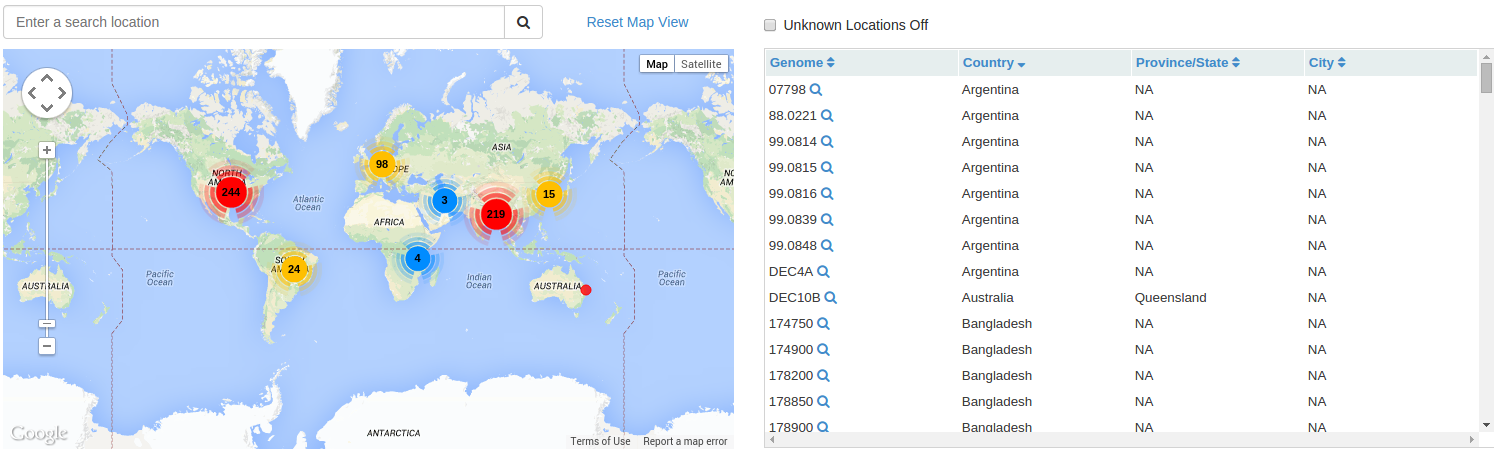
\includegraphics[scale=0.36]{../manuscript_images/map.png}

\end{landscape}

\pagebreak

\begin{landscape}

For ease of access, each map comes with a quick search, that will pan and zoom to a location of interest. The accompanying map table will update the list of genomes currently in the map view port. As an example here we show the map when a user searches for "United Kingdom":\\

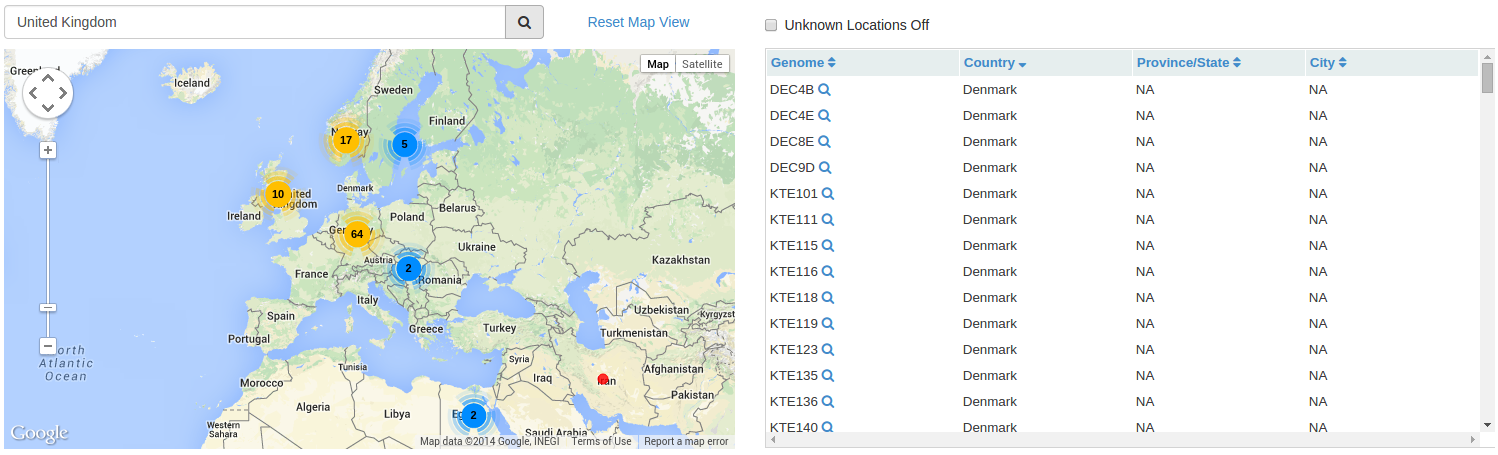
\includegraphics[scale=0.36]{../manuscript_images/uk-map.png}

\end{landscape}

%%
\section{Maps in Search}

Maps are highly integrated with Superphy's genome search and filtering controls, and this feature is designed to work seamlessly across all components of the website. The filtering system will only show map markers and genomes on the map table that are part of the filter/search query. Therefore, users can quickly and easily identify and select genomes with particular attributes, isolated from a region of interest, before querying deeper information about the genome(s) of interest. Users can also add additional sortable metadata fields to the map table by selecting from the list of check boxes in the metadata side control panel. 

\pagebreak

\begin{landscape}

%%
\section{Maps in Genome Information}

Maps are used to highlight geospatial information about genomes. Once a user has requested information about a particular genome they are directed to a page that contains a detailed overview of that genome. If there is location data available a distinct marker is displayed on the map and genome is highlighted in the map table. Maps are designed such that users can quickly jump to another genome info page right from the map table.\\

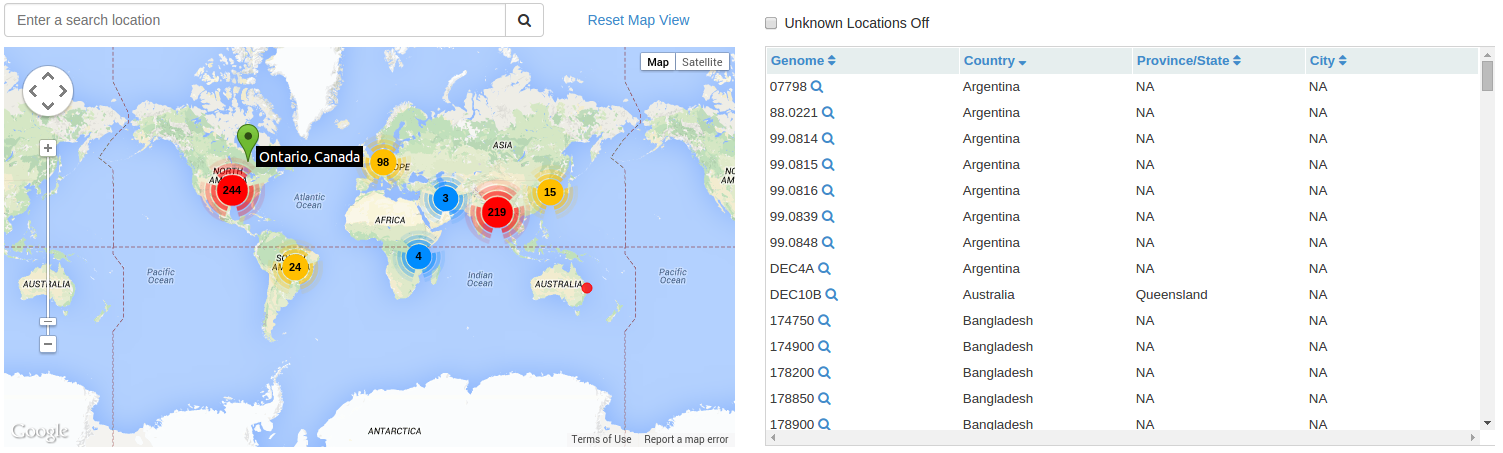
\includegraphics[scale=0.36]{../manuscript_images/genome-info.png}

\end{landscape}

%%
\section{Maps in Geospatial-Phylogeny Information}

Superphy's interactive phylogenetic tree is a powerful visual tool for discerning evolutionary relationships between genomes. Synchronizing the tree and map into a single view (GeoPhy) allows users to view these evolutionary relationships across space and time, and can potentially answer interesting scientific and epidemiological questions. Filter and search features are also built directly into GeoPhy allowing users to execute deep queries.

As an example, a user can search for a particular clade of genomes in the tree and view geospatial arrangements to discern if they were part of an outbreak, or they may select genomes isolated from a particular host and location and view their phylogenetic relationships.

\pagebreak

\begin{landscape}

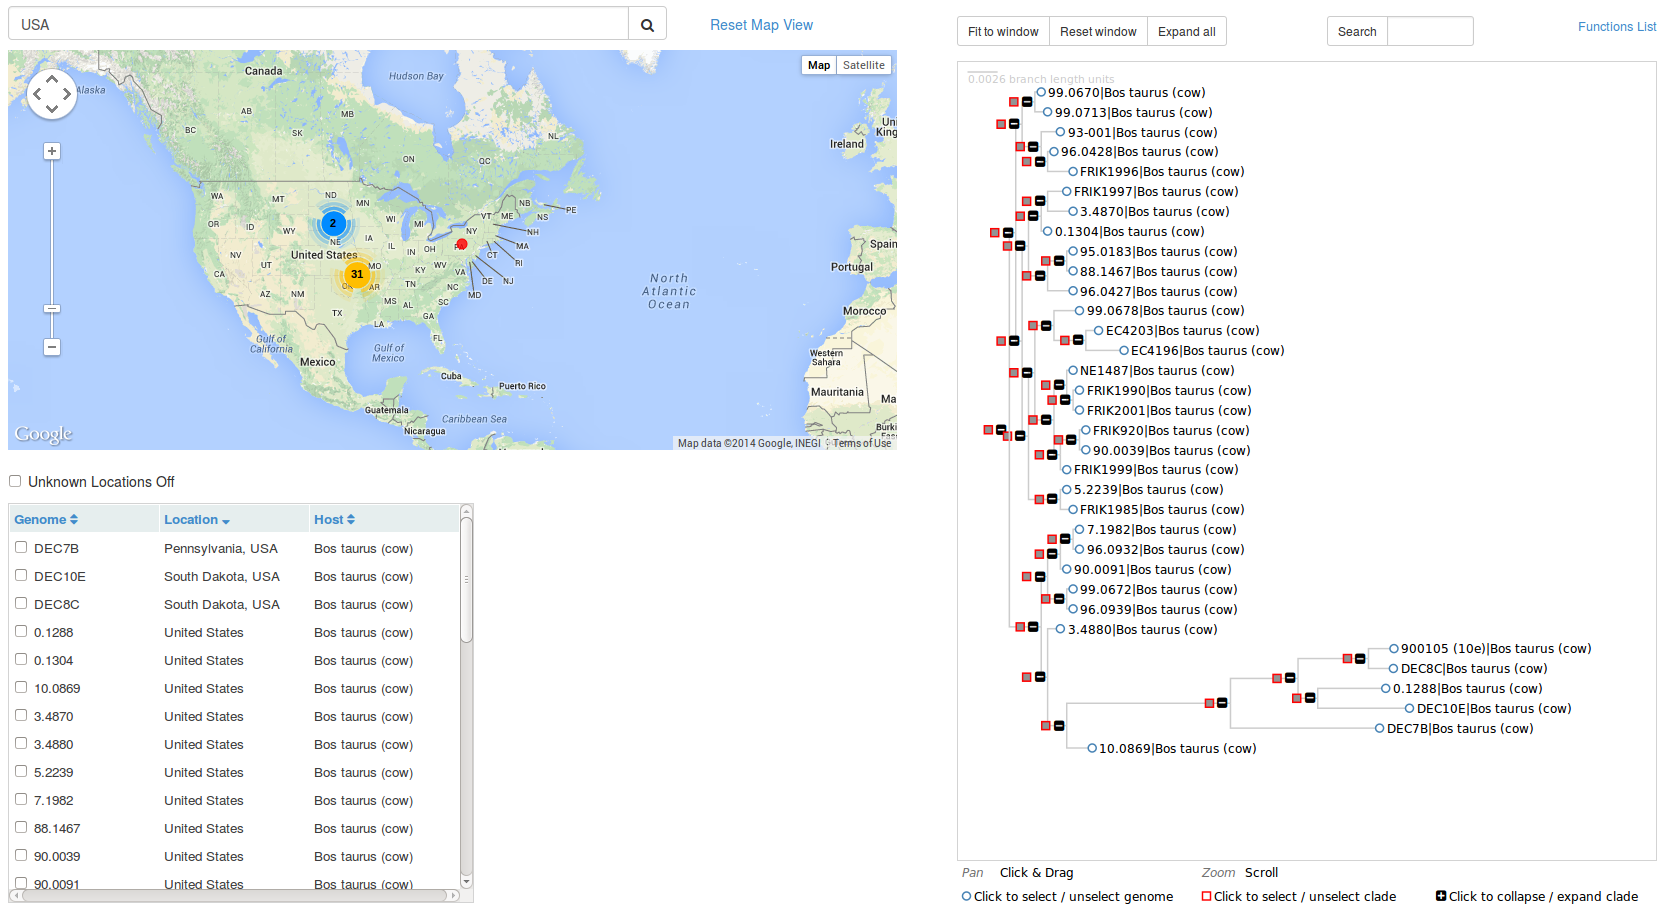
\includegraphics[scale=0.33]{../manuscript_images/geophy.png}

\end{landscape}


\end{document}